\documentclass[border=8pt]{standalone}
% Shared preamble for IronClaw thesis figures (standalone TikZ).
\renewcommand{\familydefault}{\sfdefault}
\usepackage{tikz}
\usetikzlibrary{arrows.meta,positioning,calc,fit,backgrounds,shapes.geometric,shapes.misc}

% IronClaw palette (matches slides.tex)
\definecolor{IronDark}{HTML}{1A2B3C}
\definecolor{IronBlue}{HTML}{2E86AB}
\definecolor{IronTeal}{HTML}{06A77D}
\definecolor{IronOrange}{HTML}{F18F01}
\definecolor{IronRed}{HTML}{C73E1D}
\definecolor{IronLight}{HTML}{F4F7F9}
\definecolor{IronGray}{HTML}{5D6D7E}

\tikzset{
  figtitle/.style={font=\large\bfseries\color{IronDark}, align=center},
  hostbox/.style={draw=IronBlue, rounded corners=5pt, fill=IronBlue!8,
                  line width=1pt, align=center, font=\small\color{white}},
  hostfill/.style={draw=IronBlue, rounded corners=4pt, fill=IronBlue,
                   line width=0.8pt, align=center, font=\small\color{white},
                   text width=3.1cm, minimum height=0.85cm},
  guestfill/.style={draw=IronOrange, rounded corners=4pt, fill=IronOrange!85,
                    line width=0.8pt, align=center, font=\small\color{white},
                    text width=3.1cm, minimum height=0.85cm},
  guestsoft/.style={draw=IronOrange, rounded corners=4pt, fill=IronOrange!25,
                    line width=0.8pt, align=center, font=\small\color{IronDark},
                    text width=3.1cm, minimum height=0.75cm},
  arrow/.style={-{Latex[length=2.6mm,width=2mm]}, line width=0.9pt, IronDark},
  biarrow/.style={{Latex[length=2.6mm,width=2mm]}-{Latex[length=2.6mm,width=2mm]},
                  line width=0.9pt, IronDark},
  note/.style={font=\footnotesize\color{IronGray}, align=center},
}

\begin{document}
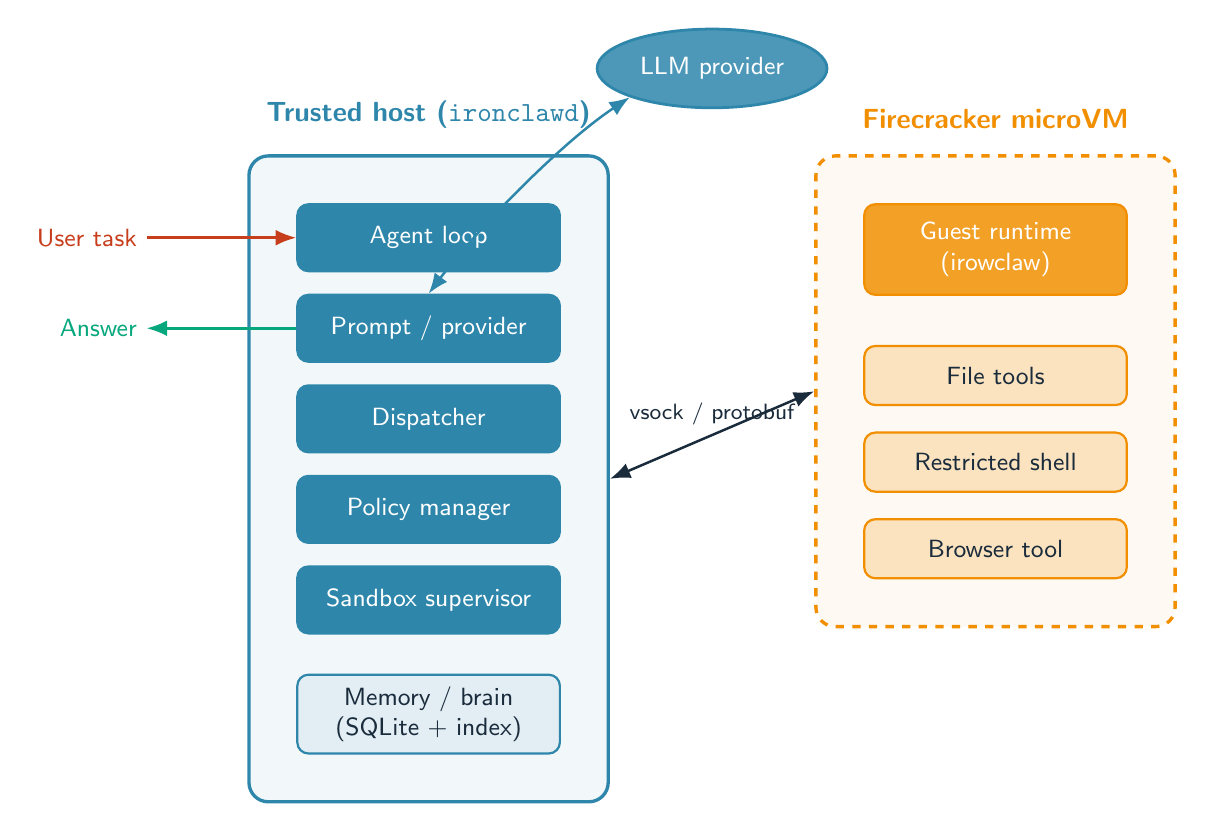
\begin{tikzpicture}

  % ---- Host daemon stack (left) ----
  \node[hostfill] (agent)  at (0,0)      {Agent loop};
  \node[hostfill] (prompt) at (0,-1.15)  {Prompt / provider};
  \node[hostfill] (disp)   at (0,-2.30)  {Dispatcher};
  \node[hostfill] (policy) at (0,-3.45)  {Policy manager};
  \node[hostfill] (super)  at (0,-4.60)  {Sandbox supervisor};
  \node[draw=IronBlue, rounded corners=4pt, fill=IronBlue!14, line width=0.8pt,
        align=center, font=\small\color{IronDark}, text width=3.1cm,
        minimum height=1.0cm] (memory) at (0,-6.05) {Memory / brain\\(SQLite + index)};

  % ---- Guest runtime stack (right) ----
  \node[guestfill, minimum height=1.15cm] (runtime) at (7.2,-0.15) {Guest runtime\\(irowclaw)};
  \node[guestsoft] (filet)  at (7.2,-1.75) {File tools};
  \node[guestsoft] (shell)  at (7.2,-2.85) {Restricted shell};
  \node[guestsoft] (browser)at (7.2,-3.95) {Browser tool};

  % ---- Containers behind the stacks ----
  \begin{scope}[on background layer]
    \node[draw=IronBlue, line width=1.2pt, rounded corners=7pt, fill=IronBlue!6,
          fit=(agent)(memory), inner sep=6mm] (hostcont) {};
    \node[draw=IronOrange, line width=1.2pt, dashed, rounded corners=7pt,
          fill=IronOrange!5, fit=(runtime)(browser), inner sep=6mm] (guestcont) {};
  \end{scope}

  % ---- Container titles (placed above, no overlap) ----
  \node[font=\normalsize\bfseries\color{IronBlue}, above=2mm of hostcont.north]
        {Trusted host (\texttt{ironclawd})};
  \node[font=\normalsize\bfseries\color{IronOrange}, above=2mm of guestcont.north]
        {Firecracker microVM};

  % ---- LLM provider ----
  \node[draw=IronBlue, line width=1pt, fill=IronBlue!85, ellipse,
        font=\small\color{white}, minimum width=2.6cm, minimum height=1.0cm]
        (llm) at (3.6,2.15) {LLM provider};

  % ---- External I/O labels ----
  \node[font=\small\color{IronRed}, left=1.9cm of agent] (utask) {User task};
  \node[font=\small\color{IronTeal}, left=1.9cm of prompt] (ans) {Answer};

  % ---- Arrows ----
  \draw[arrow, IronRed]  (utask.east) -- (agent.west);
  \draw[arrow, IronTeal] (prompt.west) -- (ans.east);
  \draw[biarrow, IronBlue] (prompt.north) .. controls +(0.6,0.8) and +(-0.9,-0.6) .. (llm.south west);
  \draw[biarrow] (hostcont.east) -- node[above, note] {vsock / protobuf} (guestcont.west);

\end{tikzpicture}
\end{document}
